\documentclass{article}
\usepackage[spanish]{babel}
\usepackage[utf8]{inputenc}
\usepackage{graphicx}
\usepackage{minted}
\usepackage{courier}
\usepackage[dvipsnames]{xcolor}
\usepackage{relsize}
\usepackage{amsmath}

\definecolor{red}{rgb}{0.95,0.12,0.14}
\definecolor{green}{rgb}{0.47,0.58,0.17}
\definecolor{darkTurquoise}{rgb}{0.18,0.65,0.74}
\definecolor{blue}{rgb}{0.16,0,0.98}
\definecolor{purple}{rgb}{0.65,0.03,0.69}

\title{\textbf{Criptografía aplicada: Cálculo del hash SHA-256 de un bloque Bitcoin}}
\author{Javier Domínguez Gómez \\
\small{jdg@member.fsf.org} \\
\small{Fingerprint: 94AD 19F4 9005 EEB2 3384 C20F 5BDC C668 D664 8E2B}}
\date{v0.1.09 - Mayo 2019}

\begin{document}
\maketitle

\tableofcontents{}

\vspace{19mm}

\section{Introducción}
    \subsection{Formatos en el texto}
    A lo largo de este documento el lector encontrará algunas palabras o bloques de texto con diferentes formatos o tipografía. Se mostrarán en letra \textit{cursiva} las palabras en inglés o que hagan referencia a algún término técnico. Resaltadas o en \textbf{negrita} aquellas palabras que describen una propiedad, una variable o un nombre de fichero, y finalmente con tipografía \texttt{Courier} aquellos datos que representen un valor hexadecimal o base 16, o fragmentos de código fuente en diferentes lenguajes de programación.
    
    \subsection{Objetivo}
    Este documento presenta en detalle un análisis criptográfico sobre cada una de las partes de las que se compone un bloque de datos en el criptosistema definido por el protocolo \textit{Bitcoin}\footnote{https://bitcoin.org/bitcoin.pdf}. Se tratarán algunos aspectos importantes como los diferentes datos, tipos, formatos y la distribución de los mismos en la estructura del bloque, así como las operaciones lógico-matemáticas de la función criptográfica SHA-256\footnote{https://github.com/JavierDominguezGomez/Cryptography/blob/master/SHA-256/Cryptography\_SHA-256\_es.pdf} que se emplean con el fin de generar un \textit{hash} resultante adecuado, es decir, un resultado que cumpla las características definidas en el protocolo \textit{Bitcoin}. Finalmente este \textit{hash} representará dicho bloque en lo que se conoce como la cadena de bloques, o como el propio creador Satoshi Nakamoto lo llamaba originalmente, \textit{timechain}\footnote{https://bitcointalk.org/index.php?topic=382374.0}. Todos los datos utilizados en los ejemplos, así como en los cálculos, son datos reales pertenecientes al bloque número \texttt{\#}286819 de la cadena de bloques de \textit{Bitcoin} en la red principal \textit{mainnet}. No existe ninguna razón especial en la elección de este bloque, es uno al azar. El lector puede consultar los datos de este o cualquier otro bloque, bien en la cadena de bloques descargada en su computadora local o bien en un \textit{explorador de bloques online}\footnote{https://www.blockchain.com/en/btc/block-height/286819}, y realizar los mismos cálculos en todos los casos, obviamente obteniendo resultados diferentes.
    
    \subsection{A quién va dirigido}
    El documento va dirigido a principalmente a lectores familiarizados con la criptología en cualquiera de sus dos ramas: la criptografía y el criptoanálisis. También va dirigido a estudiantes de ciencias de la computación o matemáticas, en general a lectores que todavía no se han adentrado en el campo de del análisis forense criptográfico sobre la información que contiene un bloque de la cadena de bloques de \textit{Bitcoin}, pero que quieren comprender su funcionamiento al más bajo nivel, a nivel de \textit{bits}. El texto trata de facilitar al lector la información sobre los métodos empleados para obtener un \textit{hash} que cumpla una serie de requisitos según el criptosistema planteado por el protocolo \textit{Bitcoin}. Para ello será necesario tener de antemano unos conocimientos mínimos sobre matemática discreta, \textit{álgebra de Boole}\footnote{https://en.wikipedia.org/wiki/Boolean\_algebra}, conversión de datos en diferentes bases como binario, decimal y hexadecimal, y comprender cómo funcionan algunas operaciones lógicas, módulo, rotativas y de desplazamiento de \textit{bits}.

\section{Estructura de datos de un bloque}
    
    \vspace{3mm}
    
    Cuando se hace referencia a un \textit{bloque} en realidad se está haciendo referencia a un conjunto de datos ordenados en base a unas normas, que en el caso que nos atañe se definen cuando se desarrolla el protocolo \textit{Bitcoin}, creando así una estructura de datos ordenada y segmentada de forma que sea sencillo identificar cada una de las partes. Los datos se ordenan en 5 secciones principales. La primera sección se reserva para un dato denominado \textbf{magicId}, un dato numérico de 4 \textit{bytes} y la segunda sección para almacenar el dato \textbf{size}, al igual que el anterior también es un dato numérico de 4 \textit{bytes}, este representará el tamaño final del bloque. En los siguientes puntos se explicará en detalle cada uno de los datos. Estos dos segmentos juntos se pueden usar como el delimitador que separa un bloque de otro en la cadena, pues los \textit{bytes} que conforman los datos de los bloques se representan concatenados uno a continuación de otro. La siguiente imagen representa la estructura de un bloque en el que se muestra resaltado en color verde el segmento que alberga el dato \textit{magicId} y en amarillo el segmento que alberga el dato \textit{size}, ambos seguidos por el resto de datos del bloque, la zona de color gris punteada.
    
    \begin{figure}[H]
    \centering
        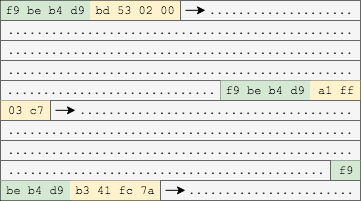
\includegraphics[scale=0.61]{img/Bitcoin_SHA_256-Block_delimitadores_de_datos.png}
        \caption{Los dos primeros segmentos de datos concatenados de cada bloque.}
    \end{figure}
    
    El tercer segmento tiene un espacio de memoria reservado de 80 \textit{bytes} para almacenar los datos de la cabecera o \textbf{header}. El cuarto segmento almacenará un dato denominado \textbf{transactionCount} que representa el número de transacciones que contiene el bloque, será un número de tipo entero sin signo y el tamaño puede variar dependiendo del número de transacciones en cada bloque. Por último, el quinto segmento se reserva para almacenar todos los datos de los que se componen cada una de las transacciones, esta sección llamada \textbf{transaction\ data} tendrá un tamaño variable que se corresponde con el tamaño disponible o restante hasta completar el bloque. A continuación una representación gráfica de los 5 segmentos de datos de los que se compone cada bloque.
    
    \begin{figure}[H]
    \centering
        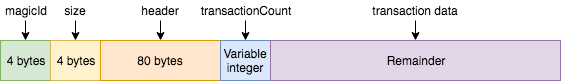
\includegraphics[scale=0.57]{img/Bitcoin_SHA_256-Block_data}
        \caption{Los 5 bloques de datos principales en cada bloque de la cadena.}
    \end{figure}
    
    El segmento \textbf{header} a su vez se compone de 6 datos que son \textbf{versionNumber}, \textbf{previousBlockHash}, \textbf{merkleRoot}, \textbf{timeStamp}, \textbf{targetDifficulty} y \textbf{nonce}. Todos los datos del bloque tienen sus propios atributos, como puede ser el tipo de dato o tipo primitivo, un nombre, el tamaño que ocupa en memoria y el formato en el que este se representará finalmente. En la siguiente tabla se categorizan los datos más significativos y a continuación se explican en detalle.
    \begin{table}[H]
    \centering
    \begin{tabular}{| c | l | c | l |} 
        \hline
        Tipo de dato & Nombre & Tamaño & Formato \\
        \hline
        uint32\_t & magicID & 4 bytes & Little-endian \\
        \hline
        uint32\_t & size & 4 bytes & Little-endian \\
        \hline
        uint32\_t & versionNumber & 4 bytes & Little-endian \\
        \hline
        uint8\_t[32] & previousBlockHash & 32 bytes & Big-endian \\
        \hline
        uint8\_t[32] & merkleRoot & 32 bytes & Big-endian \\
        \hline
        uint32\_t & timeStamp & 4 bytes & Little-endian \\
        \hline
        uint32\_t & targetDifficulty & 4 bytes & Little-endian \\
        \hline
        uint32\_t & nonce & 4 bytes & Little-endian \\
        \hline
        uint8/16/32/64\_t & transactionCount & 1, 3, 5 o 9 bytes & Big-endian*  \\
        \hline
    \end{tabular}
    \caption{Principales datos de un bloque en la cadena de bloques de \textit{Bitcoin}.}
    \label{table:0}
    \end{table}
    
    \begin{enumerate}
        \item \textbf{magicID}: En la red de \textit{Bitcoin} se establecen conexiones entre los nodos con la finalidad de establecer una comunicación para el envío y recepción de datos o mensajes. Los mensajes se envían mediante un canal en el que según van llegando se van concatenando uno detrás de otro. Así pues, cuando se desarrolló el protocolo \textit{Bitcoin} se vio conveniente añadir un prefijo en cada mensaje anteponiendo este dato de 4 \textit{bytes} y así poder identificar fácilmente no solo la red de \textit{Bitcoin} en la que se generan, si no también dónde empieza y termina cada mensaje que circula entre los diferentes nodos de la red. La siguiente tabla muestra los diferentes valores que puede tener la variable \textit{magicID} dependiendo de la red.
        
        \begin{table}[H]
        \centering
        \begin{tabular}{| c | c |} 
            \hline
            Red & magicID \\
            \hline
            Mainnet & \texttt{0xf9beb4d9} \\
            \hline
            Testnet & \texttt{0xfabfb5da} \\
            \hline
            Testnet3 & \texttt{0x0b110907} \\
            \hline
            Namecoin & \texttt{0xf9beb4fe} \\
            \hline
            Regtest & \texttt{0xfabfb5da} \\
            \hline
        \end{tabular}
        \label{table:1}
        \end{table}
        
        Se decidió establecer estos valores tan específicos dada la improbabilidad de que los caracteres ASCII que representan se encuentren en un mensaje estándar, tal y como se indica en el archivo \textit{chainparams.cpp}\footnote{https://github.com/bitcoin/bitcoin/blob/master/src/chainparams.cpp\#L99} que lo implementa en el código de \textit{Bitcoin}.
    
        \item \textbf{size}: En un dato numérico hexadecimal de 4 \textit{bytes} de valor variable que representa la longitud en \textit{bytes} del bloque actual. Está codificado en formato \textit{Little-endian}. Por ejemplo, un bloque con tamaño 152.509 KB tendrá el siguiente valor:
        
        \begin{figure}[H]
        \centering
            $152509_{10} = \texttt{0x000253BD} \Rightarrow \texttt{0xBD530200}$
        \end{figure}
        
        \item \textbf{versionNumber}: Este dato hexadecimal puede cambiar de valor cuando se actualiza el software y cambia el número de la versión del protocolo. Tiene un tamaño de 4 \textit{bytes} y se codifica en formato \textit{Little-endian}, por ejemplo:
        
        \begin{figure}[H]
        \centering
            $2_{10} = \texttt{0x00000002} \Rightarrow \texttt{0x02000000}$
        \end{figure}
        
        \item \textbf{previousBlockHash}: Se trata del \textit{hash} o \textit{digest} resultante del bloque anterior tras aplicar las funciones criptográficas utilizando los datos de la cabecera de dicho bloque. Tiene una longitud de 256 \textit{bits} o 32 \textit{bytes} codificado en formato \textit{Big-endian}. Tal y como se explica al inicio del este documento el ejemplo en todo caso toma los datos correspondientes al bloque \texttt{\#}286819, así pues, el valor de este dato ha de ser el \textit{hash} resultante del bloque anterior, que en este caso es el bloque \texttt{\#}286818\footnote{https://blockstream.info/block/000000000000000117c80378b8da0e33559b5997f2ad55e2f7d18ec1975b9717}.
        
        \begin{figure}[H]
        \centering
        \scriptsize{
            \texttt{000000000000000117c80378b8da0e33559b5997f2ad55e2f7d18ec1975b9717}
        }
        \end{figure}
        
        \item \textbf{merkleRoot}: Cada vez que una nueva transacción es aceptada el valor de esta variable se modifica. Se trata de un \textit{hash} hexadecimal de 32 \textit{bytes} codificado en formato \textit{Big-endian}. Para obtener el \textit{hash} final, también llamado \textit{hash root} se han de concatenar los datos de las transacciones ubicados en los nodos hoja del árbol, en grupos de dos. De ese modo, por cada dos transacciones se obtiene un \textit{hash} nuevo que será incluido en un nuevo vector que repetirá la acción hasta llegar al \textit{hash root}.
        
        \begin{figure}[H]
        \centering
            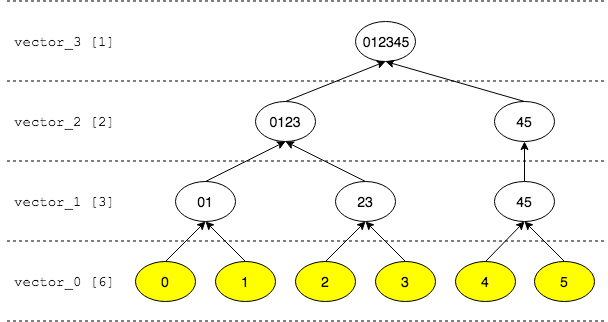
\includegraphics[scale=0.53]{img/Merkle_tree_05_leaves_nodes}
            \caption{Ejemplo de árbol de Merkle con 5 nodos hoja}
        \end{figure}
        
        Cada uno de los vectores $\mathbf{v} \ = \langle v_{1}, v_{2}, \dots, v_{n - 1}, v_{n} \rangle$ irá reduciendo el numero de nodos o elementos mediante la siguiente función recursiva por intervalos o algoritmo de complejidad $O(n)$.
        
        \begin{figure}[H]
        \centering
            $f(\mathbf{v}) = \mathlarger{\sum}_{i=0}^{n} \left \{
            \begin{array}{ll}
                \langle \mathbf{v}^{\prime}, v_{i}\rangle & \mbox{si } i=n-1 \\
                \langle \mathbf{v}^{\prime}, v_{i}||v_{i+1} \rangle & \mbox{si } i < n \\
                i+2
            \end{array}
            \right .$
        \end{figure}
        A continuación un ejemplo escrito en lenguaje C++ que implementa dicho algoritmo\footnote{https://github.com/JavierDominguezGomez/Cryptography/blob/master/MerkleTree/merkleTree.cpp}:
        
        \begin{minted}[fontsize=\small]{cpp}
#include <iostream>
#include <sstream>
#include <vector>
#include "sha256.h"
 
using namespace std;
 
void printVector(vector<string>);
string merkleTree(vector<string>);
string merkleTreeRoot;
 
int main(int argc, char *argv[]) {
    string msg = argv[1];
    istringstream buf(msg);
    vector<string> leafNodesV;
    
    for (string node; buf >> node;)
        leafNodesV.push_back(sha256(node));
        
    printVector(leafNodesV);
    cout << "Root: " << merkleTree(leafNodesV) << endl;
    
    return 0;
}

string merkleTree(vector<string> v) {
    if (v.size() > 1) {
        vector<string> aux;
        int i;
        
        for (i = 0; i < v.size(); i += 2) {
            if (i == v.size() - 1) {
                aux.push_back(v[i]);
            } else if (i < v.size()) {
                aux.push_back(sha256(v[i] + v[i + 1]));
            }
        }
        merkleTree(aux);
    } else if(v.size() == 1){
        merkleTreeRoot = v[0];
    }
    
    return merkleTreeRoot;
}

void printVector(vector<string> v) {
    cout << "v.size() = " << v.size() << endl;
    int i = 0;
    while (i < v.size()) {
        cout << "v[" << i << "]: " << v[i] << endl;
        i++;
    }
}
        \end{minted}
        
        \item \textbf{timeStamp}: Se trata de un número entero sin signo de 4 \textit{bytes} también llamado \textit{Epoch} o \textit{Tiempo Unix}. Representa el número de segundos que han transcurrido desde el 1 de enero de 1970 a las 00:00:00. Se codifica en formato \textit{Little-endian}.
        
        Un ejemplo de cómo se puede calcular este dato es mediante el siguiente código\footnote{https://github.com/JavierDominguezGomez/Cryptography/blob/master/tools/date2epoch.c} escrito en lenguaje C. Nótese que las horas se procesan como \textit{GMT+1}.
        
        \begin{minted}[fontsize=\small]{c}
#include <stdio.h>
#include <time.h>

int main(int argc, char *argv[]) {
    int year, month, day, hour, minute, second;
    struct tm t;
    time_t tod;
    
    printf("Year: ");
    scanf("%d", &year);
    printf("Month: ");
    scanf("%d", &month);
    printf("Day: ");
    scanf("%d", &day);
    printf("Hour: ");
    scanf("%d", &hour);
    printf("Minute: ");
    scanf("%d", &minute);
    printf("Second: ");
    scanf("%d", &second);
    
    t.tm_year = year - 1900;
    t.tm_mon = month - 1;   // Values [0-11]
    t.tm_mday = day;
    t.tm_hour = hour + 1;   // GMT+1
    t.tm_min = minute;
    t.tm_sec = second;
    t.tm_isdst = 0;         // DST = 0
    tod = mktime(&t);
    
    printf("Timestamp epoch: %ld\n", (long) tod);
}
        \end{minted}
        
    
        \item \textbf{targetDifficulty}: A este dato también se le llama simplemente \textit{target} o "\textit{Bits}" si se hace referencia al empaquetado de datos en el bloque. Se trata de un número entero de 256 \textit{bits} representado como un número decimal muy grande, tanto que abarcaría el rango de números existentes entre $0$ y $2^{256}-1$. El siguiente número sería el valor hexadecimal máximo que podría tomar la variable \textit{targetDifficulty}.
        
            \begin{figure}[H]
                \centering
                \scriptsize{
                $\texttt{0x}\underbrace{\texttt{00000000ffffffffffffffffffffffffffffffffffffffffffffffffffffffff}}_{256\ bits}$
                }
            \end{figure}
        
        En el bloque se almacena como un número decimal de coma flotante truncando, por ejemplo, el valor hexadecimal anterior quedaría representado de la siguiente forma.
        
            \begin{figure}[H]
                \centering
                \scriptsize{
                $\texttt{0x}\underbrace{\texttt{00000000ffff0000000000000000000000000000000000000000000000000000}}_{256\ bits}$
                }
            \end{figure}
        
        La dificultad es el resultado de dividir el valor máximo entre el valor actual de la variable \textit{targetDifficulty}, tal y como se muestra en la siguiente fórmula.
        
            \begin{figure}[H]
                \centering
                $Dificultad = \cfrac{target \ maximo}{target \ actual} = \cfrac{\texttt{0x00000000ffff0000...00}}{\texttt{0x0000000019015f53...00}}$
            \end{figure}
        
        A continuación un fragmento de código escrito en lenguaje C++ que realiza el cálculo y que se puede emplear para hallar la dificultad de minado\footnote{https://en.bitcoin.it/wiki/Difficulty}.
        
        \begin{minted}[fontsize=\small]{c}
#include <iostream>
#include <cmath>

inline float fast_log(float val)
{
   int * const exp_ptr = reinterpret_cast <int *>(&val);
   int x = *exp_ptr;
   const int log_2 = ((x >> 23) & 255) - 128;
   x &= ~(255 << 23);
   x += 127 << 23;
   *exp_ptr = x;

   val = ((-1.0f/3) * val + 2) * val - 2.0f/3;
   return ((val + log_2) * 0.69314718f);
}

float difficulty(unsigned int bits)
{
    static double max_body = fast_log(0x00ffff),
                             scaland = fast_log(256);
    return exp(max_body - fast_log(bits & 0x00ffffff) +
               scaland * (0x1d - ((bits & 0xff000000) >> 24)));
}

int main()
{
    std::cout << difficulty(0x19015f53) << std::endl;
    return 0;
}
        \end{minted}
        
        Hay que tener en cuenta el valor de la variable \textit{targetDifficulty} en cada caso, por ejemplo en el bloque \texttt{\#}286819 dicho valor es \texttt{0x19015f53}. Es una de las variables más importantes a tener en cuenta a la hora de obtener el \textit{hash} adecuado del bloque antes de incorporarlo a la cadena como un bloque válido. Así pues la prueba de trabajo o \textit{Proof of Work} tendrá mayor o menor dificultad. En el protocolo de \textit{Bitcoin} se define una regla que dice que el \textit{hash} del bloque ha de ser un número menor o igual al valor de esta variable \textit{targetDifficulty} en ese momento. De modo que si el \textit{hash} obtenido como candidato a generar un bloque fuese un número menor o igual al de \textit{targetDifficulty} habría posibilidades para que el \textit{hash} candidato sea válido para generar un nuevo bloque, aunque de forma adicional se han de cumplir otras condiciones. Por el contrario, si el \textit{hash} obtenido como candidato fuera un número mayor que el valor de esta variable \textit{targetDifficulty}, este quedaría desestimado, entonces habría que incrementar el valor de la variable \textit{nonce} y repetir todo el proceso para generar un \textit{hash} nuevo. El siguiente gráfico\footnote{http://bitcoin.sipa.be/} muestra la variación de la dificultad a lo largo del tiempo.
        
        \begin{figure}[H]
        \centering
            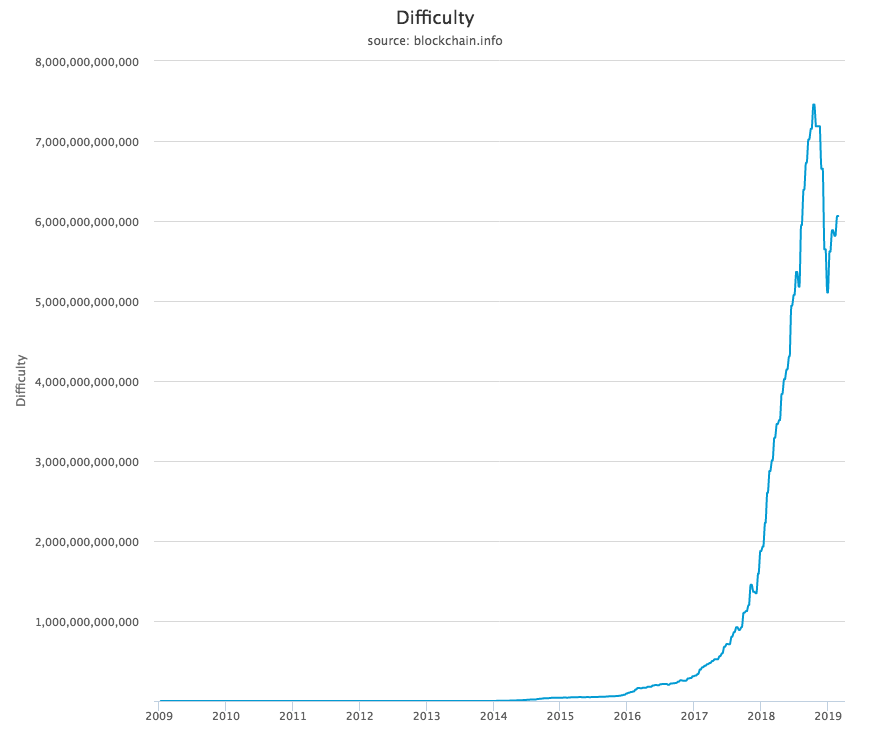
\includegraphics[scale=0.51]{img/Bitcoin_TargetDifficulty.png}
            \caption{Dificultad de minado desde enero de 2009 hasta hoy.}
        \end{figure}
        
        El valor de la variable \textit{targetDifficulty} se modifica automáticamente una vez se han generado 2016 bloques, esto sucede aproximadamente cada dos semanas. El nuevo valor se obtiene mediante un cálculo que realizan todos los clientes \textit{Bitcoin} de la red en el que toman el tiempo real que ha llevado generar los 2016 bloques y se obtiene la diferencia porcentual respecto al número de bloques que se esperaba haber calculado en el periodo de dos semanas. Cuanto menor sea el valor de la variable \textit{targetDifficulty} más aumentará la dificultad para hallar un \textit{hash} válido para el bloque.
        
        \item \textbf{nonce}: Se trata de un número entero sin signo aleatorio con una longitud de 32 \textit{bits} o 4 \textit{bytes} codificado en formato \textit{Little-endian}. Es el dato que ha de cambiarse tras un intento fallido por encontrar el \textit{hash} del bloque adecuado, de modo que al incrementalo se han de realizar de nuevo todos los cálculos de la función SHA-256 teniendo en cuenta el nuevo valor de esta variable. Siguiendo con el ejemplo del bloque \texttt{\#}286819, este se incorporó a la cadena de bloques con un valor decimal o base 10 para la variable \textit{nonce} de $856192328$, lo que indica casi con total seguridad que se tuvieron que realizar bastantes intentos.
        
        \item \textbf{transactionCount}: En el caso de \textit{transactionCount} el tipo de dato es un entero sin signo de longitud variable. Como el propio nombre indica, dependiendo del número de transacciones que han sido procesadas tendrá un valor numérico u otro.
        
        *Cuando se le asigna por valor un entero muy grande se codifica en formato \textit{Little-endian}.
    \end{enumerate}
    
    \subsection{Datos de la cabecera o header}
    La siguiente imagen es una captura de pantalla de los datos del bloque $\#286819$ visualizados en un explorador de bloques. Se han resaltado los datos que forman parte de la cabecera o \textit{header} del bloque.
    \begin{figure}[H]
    \centering
        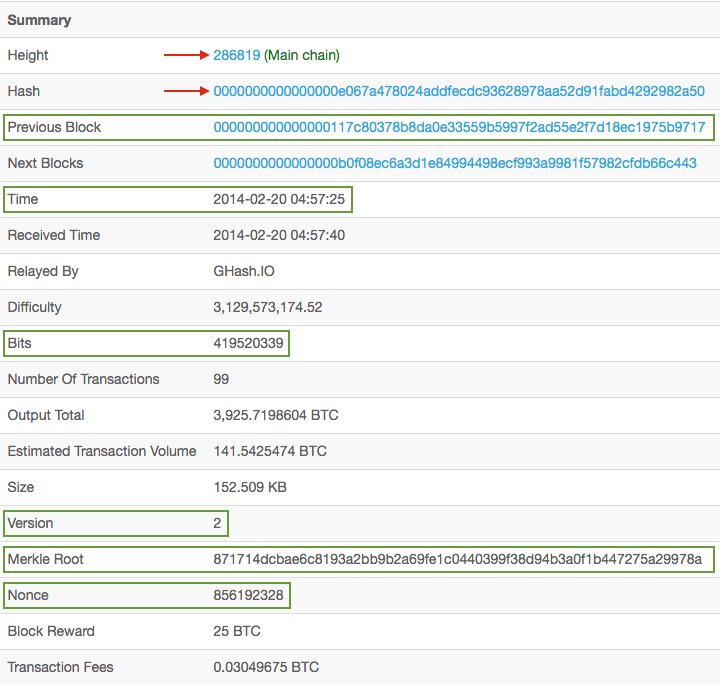
\includegraphics[scale=0.39]{img/Bitcoin_block_SHA_256_Block_Data}
        \caption{Datos empleados para la obtención del \textit{hash} del bloque \#$286819$.}
    \end{figure}
    
    \vspace{3mm}
    
\section{Construcción de la cadena de entrada M}
    Siguiendo con el ejemplo del bloque $\#286819$ de la cadena de bloques de \textit{Bitcoin}, dicho bloque está representado mediante el siguiente \textit{hash}.
    
    \begin{figure}[H]
        \centering
        \scriptsize{
        \texttt{0000000000000000e067a478024addfecdc93628978aa52d91fabd4292982a50}
        }
    \end{figure}
    
    A continuación los datos correspondientes a la cabecera o \textit{header} del bloque:
    \begin{figure}[H]
    \centering
    \scriptsize{
        $\begin{array}{ll}
            \texttt{Version:} & \texttt{2} \\
            \texttt{Prev. Block:} & \texttt{000000000000000117c80378b8da0e33559b5997f2ad55e2f7d18ec1975b9717} \\
            \texttt{Merkle root:} & \texttt{871714dcbae6c8193a2bb9b2a69fe1c0440399f38d94b3a0f1b447275a29978a} \\
            \texttt{Timestamp:} & \texttt{2014-02-20 04:57:25 (Epoch timestamp: 1392872245)} \\
            \texttt{Bits:} & \texttt{419520339} \\
            \texttt{Nonce:} & \texttt{856192328} \\
        \end{array}$
    }
    \end{figure}
    
    En este punto hay que pasar los datos en formato decimal a formato hexadecimal, de modo que quedarían de la siguiente manera:
    \begin{figure}[H]
    \centering
    \scriptsize{
        $\begin{array}{ll}
            \texttt{Version:} & \texttt{00000002} \\
            \texttt{Prev. Block:} & \texttt{000000000000000117c80378b8da0e33559b5997f2ad55e2f7d18ec1975b9717} \\
            \texttt{Merkle root:} & \texttt{871714dcbae6c8193a2bb9b2a69fe1c0440399f38d94b3a0f1b447275a29978a} \\
            \texttt{Timestamp:} & \texttt{53058B35} \\
            \texttt{Bits:} & \texttt{19015F53} \\
            \texttt{Nonce:} & \texttt{33087548} \\
        \end{array}$
    }
    \end{figure}
    
    Ahora hay que reorganizar los datos en formato \textit{Little-Endian}:
    \begin{figure}[H]
    \centering
    \scriptsize{
        $\begin{array}{ll}
            \texttt{Version:} & \texttt{02000000} \\
            \texttt{Prev. Block:} & \texttt{17975b97c18ed1f7e255adf297599b55330edab87803c8170100000000000000} \\
            \texttt{Merkle root:} & \texttt{8a97295a2747b4f1a0b3948df3990344c0e19fa6b2b92b3a19c8e6badc141787} \\
            \texttt{Timestamp:} & \texttt{358B0553} \\
            \texttt{Bits:} & \texttt{535F0119} \\
            \texttt{Nonce:} & \texttt{48750833} \\
        \end{array}$
    }
    \end{figure}
    
    Finalmente se concatenan uno a continuación de otro, empezando por \textit{version}, seguido del \textit{hash} del bloque anterior, \textit{merkle root}, \textit{timestamp}, \textit{bits} y \textit{nonce}, formando una cadena de entrada $M$ de 160 carácteres hexadecimales con con un tamaño total de 640 \textit{bits}.
    
    \begin{figure}[H]
    \centering
        $\begin{array}{rcl}
             M & = & \left \{
            \begin{array}{c}
                \texttt{0200000017975b97c18ed1f7e255adf2} \\
                \texttt{97599b55330edab87803c81701000000} \\
                \texttt{000000008a97295a2747b4f1a0b3948d} \\
                \texttt{f3990344c0e19fa6b2b92b3a19c8e6ba} \\
                \texttt{dc141787358b0553535f011948750833}
            \end{array}
            \right .
        \end{array}$
    \end{figure}
    
    Se segmenta la cadena de entrada $M$ en bloques de 32 \textit{bits}:
    \begin{figure}[H]
    \centering
        $\begin{array}{rcl}
             M & = & \left \{
            \begin{array}{c}
                \texttt{02000000 + 17975b97 + c18ed1f7 + e255adf2} \\
                \texttt{97599b55 + 330edab8 + 7803c817 + 01000000} \\
                \texttt{00000000 + 8a97295a + 2747b4f1 + a0b3948d} \\
                \texttt{f3990344 + c0e19fa6 + b2b92b3a + 19c8e6ba} \\
                \texttt{dc141787 + 358b0553 + 535f0119 + 48750833}
            \end{array}
            \right .
        \end{array}$
    \end{figure}
    
    De este modo se obtiene el mensaje de entrada $M$. Se ha de reservar este dato para utilizarlo más adelante en la función SHA-256 como \textit{input} en la primera ronda.
    
    \subsection{Longitud de la cadena de entrada $M$}
        Una vez que se ha obtenido la cadena de entrada $M$ en el punto anterior es necesario calcular la longitud de la misma en formato hexadecimal o base 16, es decir, 640 \textit{bits} que se representan con el valor 280 en hexadecimal.
        \begin{figure}[H]
        \centering
            $|M| = \texttt{280}_{16}\ (640\ bits\ del\ mensaje\ original\ en\ hexadecimal)$
        \end{figure}
        Este dato se ha de reservar para el siguiente punto, ya que será necesario para completar los registros $W_{14}$ y $W_{15}$ de la variable $W_t$ solo en la segunda y tercera ejecución de la función SHA-256.
    
    \subsection{La variable $W_t$}
        Tal y como se describe en el punto 3 del documento "\textit{Criptografíıa aplicada: Función SHA-256}"\footnote{https://github.com/JavierDominguezGomez/Cryptography/blob/master/SHA-256/Cryptography\_SHA-256\_es.pdf}, la variable $W_{t}$ es un vector de 64 elementos que contiene palabras hexadecimales de 32 \textit{bits}. Tiene un tamaño o longitud de 2048 \textit{bits} (256 \textit{bytes}) y se obtiene mediante la siguiente función recursiva definida por intervalos.
            \begin{figure}[H]
            \centering
                $W_{t} = \left \{
                \begin{array}{lcl}
                    M_{i} & si & 0 \le i < 16 \\
                    \sigma_{1}(W_{i-2})+W_{i-7}+\sigma_{0}(W_{i-15})+W_{i-16} & si & 16 \le i < 64
                \end{array}
                \right .$
            \end{figure}
        En la anterior función recursiva definida por intervalos, el primer intervalo es el que abarca los 16 primeros registros, o sea desde $W_{0}$ hasta $W_{15}$. El segundo intervalo es el esquema de los 48 registros restantes, es decir, desde $W_{16}$ hasta $W_{63}$.
            \begin{figure}[H]
            \centering
                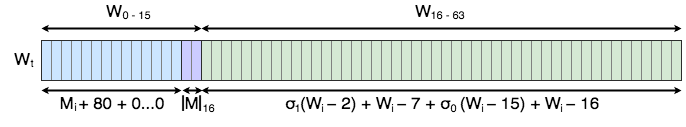
\includegraphics[scale=0.5]{img/SHA-256-Wt.png}
                \caption{Representación gráfica de $W_{t}$}
            \end{figure}
        Las funciones $\sigma_{0}$ y $\sigma_{1}$ realizan las siguientes operaciones lógicas de compresión con cada uno de los \textit{bits} de la palabra almacenada en el segmento de $W_t$ que procesan.
        \begin{figure}[H]
        \centering
            $\begin{array}{l}
                \sigma_{0}(x) = ROT \ R^{7}(x) \oplus ROT \ R^{18}(x) \oplus SHR^{3}(x) \\
                \sigma_{1}(x) = ROT \ R^{17}(x) \oplus ROT \ R^{19}(x) \oplus SHR^{10}(x)
            \end{array}$
        \end{figure}
        
        Para hallar el valor de cualquiera de los segmentos que van desde $W_{16}$ hasta $W_{63}$ se han de realizar las siguientes operaciones, donde $i$ tiene por valor el valor de $t$ en el segmento que se quiere calcular de $W_t$. Por ejemplo, para $W_{16}$:
        
        \begin{figure}[H]
        \centering
            $\sigma_{1}(W_{i-2})+W_{i-7}+\sigma_{0}(W_{i-15})+W_{i-16}$ \\
            $\Downarrow$ \\
            $\sigma_{1}(W_{16-2})+W_{16-7}+\sigma_{0}(W_{16-15})+W_{16-16}$ \\
            $\Downarrow$ \\
            $\sigma_{1}(W_{14})+W_{9}+\sigma_{0}(W_{1})+W_{0}$
        \end{figure}
        
        En este ejemplo los segmentos $W_{14}$, $W_{9}$, $W_{1}$ y $W_{0}$ de la primera ronda (\textit{Ronda \texttt{\#}0}) tienen asignados los siguientes valores:
        \begin{figure}[H]
        \centering
            $\begin{array}{rl}
                W_{14} = \texttt{0xb2b92b3a} & W_{9} = \texttt{0x8a97295a} \\
                W_{1}\  = \texttt{0x17975b97} & W_{0} = \texttt{0x02000000}
            \end{array}$
        \end{figure}
        
        A continuación se muestra una representación gráfica la operación lógica de compresión $\sigma_{1}$, que aplica sobre el valor del segmento $W_{14}$.
        
        \begin{figure}[H]
        \centering
            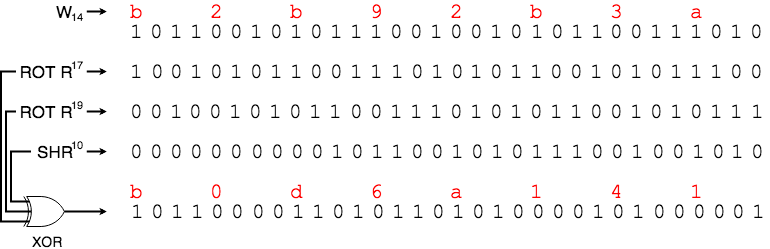
\includegraphics[scale=0.445]{img/SHA-256-Wt_operacion_sigma1.png}
            \caption{Operación $ROT \ R^{17}(x) \oplus ROT \ R^{19}(x) \oplus SHR^{10}(x)$ con cada \textit{bit}.}
        \end{figure}
        
        Tras el cálculo de $\sigma_{1}(W_{14})$ se obtiene la palabra hexadecimal de 32 \textit{bits} $\texttt{0xb0d6a141}$. Se ha de reservar este valor para calcular el resultado final. También se muestra la la representación gráfica la operación lógica de compresión $\sigma_{0}$, que aplica sobre el valor del segmento $W_{1}$.
        
        \begin{figure}[H]
        \centering
            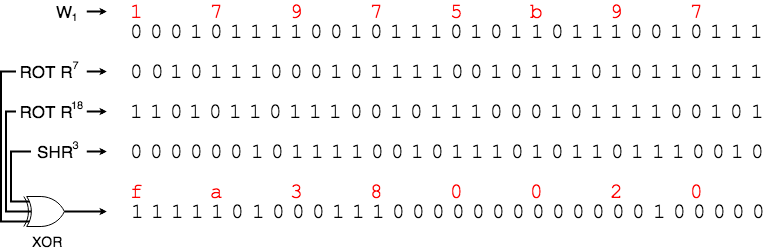
\includegraphics[scale=0.445]{img/SHA-256-Wt_operacion_sigma0.png}
            \caption{Operación $ROT \ R^{7}(x) \oplus ROT \ R^{18}(x) \oplus SHR^{3}(x)$ con cada \textit{bit}.}
        \end{figure}
        
        Tras el cálculo de $\sigma_{0}(W_{1})$ se obtiene la palabra hexadecimal de 32 \textit{bits} $\texttt{fa380020}$. Una vez realizados los cálculos necesarios para obtener el valor de $\sigma_{1}(W_{14})$ y $\sigma_{0}(W_{1})$ finalmente se ha de realizar la siguiente operación final.
        
        \begin{figure}[H]
        \centering
            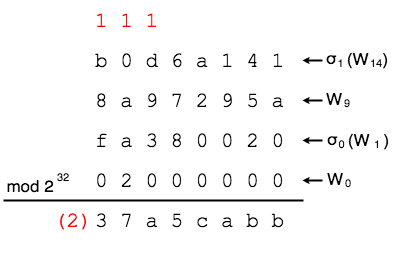
\includegraphics[scale=0.445]{img/SHA-256-Wt_operacion_mod2_32_final.png}
            \caption{Operación final $mod \ 2^{32} (\sigma_{1}(W_{14}), W_{9}, \sigma_{0}(W_{1}), W_{0})$.}
        \end{figure}
        
        De este modo se obtiene el valor que se almacenará en el segmento $W_{16}$ del vector $W_t$. Será necesario repetir el mismo proceso por cada uno de los segmentos hasta llegar a $W_{63}$.
        
        \vspace{3mm}
        
        Todos los cálculos anteriores también aplican a las reglas criptográficas de los bloques en el protocolo \textit{Bitcoin}, solo que hay que tener en cuenta que la cadena de entrada $M$ en cada bloque tiene una longitud superior a 512 \textit{bits}, lo que implica utilizar la función \textit{hash} SHA-256 tres veces, una por cada ronda, y el valor de la longitud de $M$ solo se aplicará en el esquema de relleno de la segunda y tercera ronda. En la primera ronda (\textit{Ronda \texttt{\#}0}) se rellenan los primeros 16 segmentos de la variable $W_t$ con todos los \textit{bytes} en hexadecimal que quepan, es decir, los primeros 512 \textit{bits} de $M$, rellenando también los segmentos $W_{14}$ y $W_{15}$. Los 128 \textit{bits} restantes de la cadena de entrada $M$ que no caben en esta primera ronda se reservan para los primeros 4 registros de $W_t$ de la segunda ronda. Tras la segunda ronda (\textit{Ronda \texttt{\#}1}) se obtiene un \textit{digest} de 256 \textit{bits} que se utiliza para rellenar los primeros 8 segmentos de $W_t$ en la tercera y última ronda (\textit{Ronda \texttt{\#}2}). La siguiente figura se detalla el contenido de los primeros 16 registros de la variable $W_{t}$ en cada una de las tres veces que se ejecutan las 64 iteraciones de la función SHA-256 para obtener el \textit{digest} en cada caso.
        \begin{figure}[H]
        \centering
            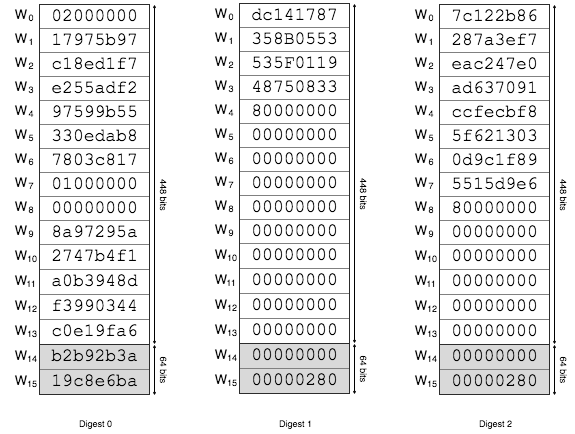
\includegraphics[scale=0.59]{img/Bitcoin_block_SHA_256_W0_W15_x3}
            \caption{Los primeros 16 registros de la variable $W_{t}$ en los tres casos en los que se ha de ejecutar la función SHA-256.}
        \end{figure}
        
        En los siguientes puntos se detalla el esquema de relleno al completo en cada una de las rondas.
        
        \subsection{Primera ronda SHA-256: Ronda 0}
        La función \textit{hash} SHA-256 realiza 64 ciclos criptográficos en los que procesará una serie de cálculos en los que tiene en cuenta por un lado las 8 palabras hexadecimales de 32 \textit{bits} asignadas como valor a las variables $A$, $B$, $C$, $D$, $E$, $F$, $G$ y $H$, y por otro lado la variable $W_t$, que es un vector de 64 elementos ordenados por intervalos. En la primera ronda criptográfica se han iniciar los
        
        \vspace{3mm}
        
        \noindent\begin{minipage}{0.23\textwidth}
        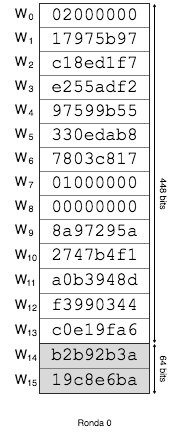
\includegraphics[scale=0.59]{img/Bitcoin_block_SHA_256_W0_W15_ronda_0}
        \end{minipage}
        \hfill
        \begin{minipage}{0.67\textwidth}
         valores de las variables $A_{0}$, $B_{0}$, $C_{0}$, $D_{0}$, $E_{0}$, $F_{0}$, $G_{0}$ y $H_{0}$ con los valores estándar de la función \textit{hash} SHA-256 en su primera iteración, es decir, los 32 primeros \textit{bits} en hexadecimal o base 16 de la parte fraccionaria de las raíces cuadradas de los primeros 8 números primos.
        
        \begin{figure}[H]
        \centering
            $\begin{array}{rr}
                A_{0} = \texttt{0x6a09e667} & B_{0} = \texttt{0xbb67ae85} \\
                C_{0} = \texttt{0x3c6ef372} & D_{0} = \texttt{0xa54ff53a} \\
                E_{0} = \texttt{0x510e527f} & F_{0} = \texttt{0x9b05688c} \\
                G_{0} = \texttt{0x1f83d9ab} & H_{0} = \texttt{0x5be0cd19}
            \end{array}$
        \end{figure}
        
        En una función SHA-256, cuando el tamaño de la cadena de entrada $M$ es igual o mayor que 512 \textit{bits} se han de rellenar los primeros 16 elementos del vector $W_t$ con los primeros 512 \textit{bits} de la cadena principal de entrada $M$, incluidos los elementos $W_{14}$ y $W_{15}$, tal y como se muestra en la imagen. El resto de la cadena $M$ se ha de reservar para la segunda ejecución de la función SHA-256 que se explicará en el siguiente punto. Teniendo la cadena $M$ de entrada, las 8 palabras
        \end{minipage}
        
        
        
        \noindent iniciales, que irán cambiando en cada una de las 64 iteraciones, y los 64 elementos del vector $W_t$ se puede comenzar a realizar las operaciones de la función SHA-256. El objetivo en esta primera ronda es obtener el primer \textit{hash}, necesario en la segunda ronda.
        
        \vspace{3mm}
        
        Cuando se hayan realizado las 64 iteraciones SHA-256 con los datos anteriores se ha de realizar una última operación en la que se ha de tomar cada palabra $A$, $B$, $C$, $D$, $E$, $F$, $G$ y $H$ de la primera iteración y realizar una operación $mod\ 2^{32}$ con su homóloga de la última iteración, véase el ejemplo.
        
        \begin{figure}[H]
        \centering
            $\begin{array}{lllll}
                \texttt{0x6a09e667}\ (A_{0}) & mod\ 2^{32} & \texttt{0x72605526}\ (A_{63}) & = & \texttt{0xdc6a3b8d} \\
                \texttt{0xbb67ae85}\ (B_{0}) & mod\ 2^{32} & \texttt{0x51019395}\ (B_{63}) & = & \texttt{0x0c69421a} \\
                \texttt{0x3c6ef372}\ (C_{0}) & mod\ 2^{32} & \texttt{0x8eab60c2}\ (C_{63}) & = & \texttt{0xcb1a5434} \\
                \texttt{0xa54ff53a}\ (D_{0}) & mod\ 2^{32} & \texttt{0x3fe7029b}\ (D_{63}) & = & \texttt{0xe536f7d5} \\
                \texttt{0x510e527f}\ (E_{0}) & mod\ 2^{32} & \texttt{0x72b36765}\ (E_{63}) & = & \texttt{0xc3c1b9e4} \\
                \texttt{0x9b05688c}\ (F_{0}) & mod\ 2^{32} & \texttt{0xb1b63303}\ (F_{63}) & = & \texttt{0x4cbb9b8f} \\
                \texttt{0x1f83d9ab}\ (G_{0}) & mod\ 2^{32} & \texttt{0x766c3d83}\ (G_{63}) & = & \texttt{0x95f0172e} \\
                \texttt{0x5be0cd19}\ (H_{0}) & mod\ 2^{32} & \texttt{0xa06805c6}\ (H_{63}) & = & \texttt{0xfc48d2df}
            \end{array}$
        \end{figure}
        
        Finalmente se concatenan los valores de los 8 resultados en esta ronda 0 obteniendo el siguiente digest resultante:
        
        \begin{figure}[H]
        \centering
            $\scriptsize{\texttt{dc6a3b8d0c69421acb1a5434e536f7d5c3c1b9e44cbb9b8f95f0172efc48d2df}}$
        \end{figure}
        Se reserva este dato para realizar la segunda ronda SHA-256 en el siguiente punto.
        
        \subsection{Segunda ronda SHA-256: Ronda 1}
        En la segunda ronda se han volver a realizar los 64 ciclos criptográficos que realiza SHA-256 teniendo en cuenta que el valor de las 8 palabras iniciales $A$, $B$, $C$, $D$, $E$, $F$, $G$ y $H$ en la primera iteración tendrán por valor inicial cada uno de los segmentos de 32 \textit{bits} correspondientes al \textit{hash} resultante de la primera ronda.
        
        \begin{figure}[H]
        \centering
            $\scriptsize{\overbrace{\texttt{dc6a3b8d}}^{A_{0}}\overbrace{\texttt{0c69421a}}^{B_{0}}\overbrace{\texttt{cb1a5434}}^{C_{0}}\overbrace{\texttt{e536f7d5}}^{D_{0}}\overbrace{\texttt{c3c1b9e4}}^{E_{0}}\overbrace{\texttt{4cbb9b8f}}^{F_{0}}\overbrace{\texttt{95f0172e}}^{G_{0}}\overbrace{\texttt{fc48d2df}}^{H_{0}}}$
        \end{figure}
        
        \begin{figure}[H]
        \centering
            $\begin{array}{rr}
                A_{0} = \texttt{0xdc6a3b8d} & B_{0} = \texttt{0xc3c1b9e4} \\
                C_{0} = \texttt{0x0c69421a} & D_{0} = \texttt{0x4cbb9b8f} \\
                E_{0} = \texttt{0xcb1a5434} & F_{0} = \texttt{0x95f0172e} \\
                G_{0} = \texttt{0xe536f7d5} & H_{0} = \texttt{0xfc48d2df}
            \end{array}$
        \end{figure}
        
        En cuanto a los primeros 16 registros de la variable $W_t$ en esta segunda ronda se se utilizarán primero los \textit{bits} del mensaje $M$ original de 640 \textit{bits} que no cabían en la ronda anterior.
        
        \vspace{3mm}
        
        \noindent\begin{minipage}{0.23\textwidth}
        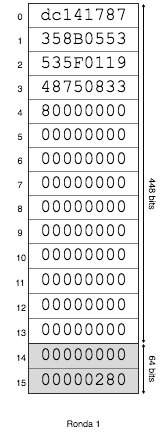
\includegraphics[scale=0.59]{img/Bitcoin_block_SHA_256_W0_W15_ronda_1}
        \end{minipage}
        \hfill
        \begin{minipage}{0.67\textwidth}
        \begin{figure}[H]
        \centering
            $\texttt{dc141787} + \texttt{358b0553} + \texttt{535f0119} + \texttt{48750833}$
        \end{figure}
        A continuación hay que tomar un \textit{bit} que represente el número 1 decimal o base 10, es decir $00000001$, este se desplaza al \textit{bit} más alto del \textit{byte}, con lo que se obtiene $10000000$ y finalmente se calcula el valor hexadecimal, que es $80$.
            \begin{figure}[H]
            \centering
                $10000000_{2} = \texttt{80}_{16}$
            \end{figure}
        Independientemente de la longitud de cadena hexadecimal de la palabra de entrada, se añade $80$ por la derecha.
            \begin{figure}[H]
            \centering
                $\texttt{486f6c61} + \texttt{206d756e} + \texttt{646f} + \texttt{80}$
            \end{figure}
        Ahora hay que añadir a la cadena una cantidad de \textit{bits} con valor $0$ hasta llegar a 448 \textit{bits} en total, que es la longitud que abarca todos los intervalos que van desde $W_{0}$ hasta $W_{13}$. Para terminar de completar los
        \end{minipage}
        
        \noindent primeros 16 segmentos de $W_{t}$ solo queda rellenar los últimos dos bloques de 32 \textit{bits} $W_{14}$ y $W_{15}$ con la longitud del mensaje de entrada $|M|$ en hexadecimal, con tantos ceros por la izquierda como sean necesario para alcanzar 64 \textit{bits} de longitud, en este caso es $280$. Los valores que irán en los segmentos desde $W_{16}$ hasta $W_{63}$ se obtienen siguiendo las pautas explicadas en el punto 6 de este documento. Al igual que en la primera ronda, cuando se hayan realizado las 64 iteraciones SHA-256 con los datos anteriores se ha de realizar una última operación en la que se ha de tomar cada palabra $A$, $B$, $C$, $D$, $E$, $F$, $G$ y $H$ de la primera iteración y realizar una operación $mod\ 2^{32}$ con su homóloga de la última iteración, véase el ejemplo.
        
        \begin{figure}[H]
        \centering
            $\begin{array}{lll}
                \texttt{0xdc6a3b8d}\ (A_0)\ mod\ 2^{32}\ \texttt{0x9fa7eff9}\ (A_63) & = & \texttt{0x7c122b86} \\
                \texttt{0x0c69421a}\ (B_0)\ mod\ 2^{32}\ \texttt{0x1c10fcdd}\ (B_63) & = & \texttt{0x287a3ef7} \\
                \texttt{0xcb1a5434}\ (C_0)\ mod\ 2^{32}\ \texttt{0x1fa7f3ac}\ (C_63) & = & \texttt{0xeac247e0} \\
                \texttt{0xe536f7d5}\ (D_0)\ mod\ 2^{32}\ \texttt{0xc82c78bc}\ (D_63) & = & \texttt{0xad637091} \\
                \texttt{0xc3c1b9e4}\ (E_0)\ mod\ 2^{32}\ \texttt{0x093d1214}\ (E_63) & = & \texttt{0xccfecbf8} \\
                \texttt{0x4cbb9b8f}\ (F_0)\ mod\ 2^{32}\ \texttt{0x12a67774}\ (F_63) & = & \texttt{0x5f621303} \\
                \texttt{0x95f0172e}\ (G_0)\ mod\ 2^{32}\ \texttt{0x77ac085b}\ (G_63) & = & \texttt{0x0d9c1f89} \\
                \texttt{0xfc48d2df}\ (H_0)\ mod\ 2^{32}\ \texttt{0x58cd0707}\ (H_63) & = & \texttt{0x5515d9e6}
            \end{array}$
        \end{figure}
        
        Finalmente se concatenan los valores de los 8 resultados en esta ronda 1 obteniendo el siguiente digest resultante:
        
        \begin{figure}[H]
        \centering
            $\scriptsize{\texttt{7c122b86287a3ef7eac247e0ad637091ccfecbf85f6213030d9c1f895515d9e6}}$
        \end{figure}
        Se reserva este dato para realizar la tercera ronda SHA-256 en el siguiente punto.
        
        \subsection{Tercera ronda SHA-256: Ronda 2}
        \noindent\begin{minipage}{0.23\textwidth}
        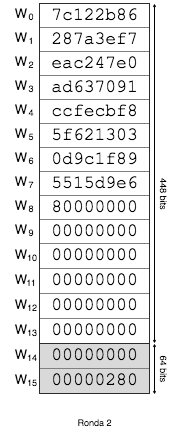
\includegraphics[scale=0.59]{img/Bitcoin_block_SHA_256_W0_W15_ronda_2}
        \end{minipage}
        \hfill
        \begin{minipage}{0.67\textwidth}
        En esta tercera ronda criptográfica (\textit{Ronda \texttt{\#}2}) se ha de utilizar como mensaje de entrada $M$ el \textit{hash} obtenido en la ronda anterior (\textit{Ronda \texttt{\#}1}). Al igual que en la ronda anterior hay que tomar un \textit{bit} que represente el número 1 decimal o base 10, es decir $00000001$, este se desplaza al \textit{bit} más alto del \textit{byte}, con lo que se obtiene $10000000$ y finalmente se calcula el valor hexadecimal, que es $80$.
            \begin{figure}[H]
            \centering
                $10000000_{2} = \texttt{80}_{16}$
            \end{figure}
        Independientemente de la longitud de cadena hexadecimal de la palabra de entrada, se añade $80$ por la derecha.
        \begin{figure}[H]
        \centering
            $\begin{array}{l}
                \texttt{7c122b86 + 287a3ef7 + eac247e0 +} \\
                \texttt{ad637091 + ccfecbf8 + 5f621303 +} \\
                \texttt{0d9c1f89 + 5515d9e6 + 80 }
            \end{array}$
        \end{figure}
        Ahora hay que añadir a la cadena una cantidad de \textit{bits} con valor $0$ hasta llegar a 448 \textit{bits} en total, que es la longitud que abarca todos los intervalos que van desde $W_{0}$ hasta $W_{13}$. Cuando se hayan realizado las
        \end{minipage}
        
        \vspace{1.3mm}
        
        \noindent 64 iteraciones SHA-256 con los datos anteriores se ha de realizar una última operación en la que se ha de tomar cada palabra $A$, $B$, $C$, $D$, $E$, $F$, $G$ y $H$ de la primera iteración y realizar una operación $mod\ 2^{32}$ con su homóloga de la última iteración, véase el ejemplo.
        
        \begin{figure}[H]
        \centering
            $\begin{array}{lllll}
                \texttt{0x6a09e667}\ (A_{0}) & mod\ 2^{32} & \texttt{0xe620b22b}\ (A_{63}) & = & \texttt{0x502a9892} \\
                \texttt{0xbb67ae85}\ (B_{0}) & mod\ 2^{32} & \texttt{0x87564c0c}\ (B_{63}) & = & \texttt{0x42bdfa91} \\
                \texttt{0x3c6ef372}\ (C_{0}) & mod\ 2^{32} & \texttt{0xf1369725}\ (C_{63}) & = & \texttt{0x2da58a97} \\
                \texttt{0xa54ff53a}\ (D_{0}) & mod\ 2^{32} & \texttt{0x82e6d493}\ (D_{63}) & = & \texttt{0x2836c9cd} \\
                \texttt{0x510e527f}\ (E_{0}) & mod\ 2^{32} & \texttt{0xadcef783}\ (E_{63}) & = & \texttt{0xfedd4a02} \\
                \texttt{0x9b05688c}\ (F_{0}) & mod\ 2^{32} & \texttt{0xdd9eff54}\ (F_{63}) & = & \texttt{0x78a467e0} \\
                \texttt{0x1f83d9ab}\ (G_{0}) & mod\ 2^{32} & \texttt{0xe07c2655}\ (G_{63}) & = & \texttt{0x00000000} \\
                \texttt{0x5be0cd19}\ (H_{0}) & mod\ 2^{32} & \texttt{0xa41f32e7}\ (H_{63}) & = & \texttt{0x00000000}
            \end{array}$
        \end{figure}
        
        Finalmente se concatenan los valores de los 8 resultados en esta ronda 0 obteniendo el siguiente digest resultante:
        
        \begin{figure}[H]
        \centering
            $\scriptsize{\texttt{502a989242bdfa912da58a972836c9cdfedd4a0278a467e00000000000000000}}$
        \end{figure}
        Para terminar, el último paso para obtener el \textit{hash} definitivo de este bloque es convertir el \textit{digest} resultante a formato \textit{Little-Endian}, tal y como se muestra a continuación.
        \begin{figure}[H]
        \centering
            $\scriptsize{\texttt{0000000000000000e067a478024addfecdc93628978aa52d91fabd4292982a50}}$
        \end{figure}
        Se puede comprobar que se cumplen los requisitos del protocolo \textit{Bitcoin} para el cálculo del \textit{hash} del bloque \texttt{\#}286819 de la cadena de bloques de \textit{Bitcoin} en la red principal \textit{mainnet}. Los datos empleados en la realización de este documento se pueden comprobar con los de la cadena de bloques de \textit{Bitcoin} desde en cualquier explorador de bloques\footnote{https://www.blockchain.com/en/btc/block-height/286819}.

\section{Almacenamiento en ficheros}
    Todos los datos de los bloques que ya han sido minados se escriben en ficheros binarios con el nombre \textbf{blk*.dat}. Estos archivos se almacenan en diferentes directorios dependiendo del sistema operativo que tenga la computadora donde se esté ejecutando el cliente \textit{Bitcoin Core}, véase la siguiente tabla:
    
    \begin{table}[H]
    \centering
    \begin{tabular}{| l | l |} 
        \hline
        Sistema operativo & Directorio \\
        \hline
        GNU/Linux y Unix & $\sim$/.bitcoin/blocks/ \\
        \hline
        MacOS & $\sim$/Library/Application Support/Bitcoin/blocks \\
        \hline
        Windows XP & \%APPDATA\%$\char`\\$Bitcoin$\char`\\$blocks \\
        \hline
        Windows Vista/7/8 & C:$\char`\\$Users$\char`\\$user$\char`\\$AppData$\char`\\$Roaming$\char`\\$Bitcoin$\char`\\$blocks \\
        \hline
    \end{tabular}
    \label{table:2}
    \end{table}
    
    \subsection{Listado y lectura de archivos}
    En este ejemplo se ha empleado un sistema operativo 100\% libre\footnote{https://www.gnu.org/distros/free-distros.es.html} GNU/Linux, así pues hay que posicionarse en el directorio $\sim$/.bitcoin/blocks/. Si se listan los archivos que contiene el directorio aparecerá una lista como la siguiente:
    
    \begin{figure}[H]
    \scriptsize{\texttt{$\sim$/.bitcoin/blocks/\$ ls -lrt \\
-rw------- 1 jdg jdg 134211184 oct  7  2018 blk00000.dat \\
-rw------- 1 jdg jdg 134182654 oct  7  2018 blk00001.dat \\
-rw------- 1 jdg jdg 134185203 oct  7  2018 blk00002.dat \\
-rw------- 1 jdg jdg 134205295 oct  7  2018 blk00003.dat \\
-rw------- 1 jdg jdg 134206001 oct  7  2018 blk00004.dat \\
-rw------- 1 jdg jdg 134215469 oct  7  2018 blk00005.dat \\
... \\
-rw------- 1 jdg jdg \ 19503795 oct  7  2018 rev00000.dat \\
-rw------- 1 jdg jdg \ 16777216 oct  7  2018 rev00002.dat \\
-rw------- 1 jdg jdg \ 16965106 oct  7  2018 rev00001.dat \\
-rw------- 1 jdg jdg \ 16777216 oct  7  2018 rev00003.dat \\
... \\
drwxr-x--- 2 jdg jdg \ \ \ \ \ 4096 oct  7 2018 index}
    }
    \end{figure}
    
    Entre todos estos archivos los que nos interesan son los que su nombre comienza por \textbf{blk} seguido de unos números y terminando con la extensión \textbf{.dat}. Al tratarse de archivos binarios no se puede leer su contenido con un editor de textos tradicional, será necesario utilizar un programa específico para tal caso, como por ejemplo el programa \textbf{hexdump}\footnote{https://www.freebsd.org/cgi/man.cgi?query=hexdump\&sektion=1}. Una vez abierto cualquiera de los archivos, por ejemplo el primer archivo \textbf{blk00000.dat}, así es como se ven los datos que contiene.
    
    \begin{figure}[H]
    \scriptsize{\texttt{$\sim$/.bitcoin/blocks/\$ hexdump -C -s 0 -n 288 blk00000.dat \\
00000000  f9 be b4 d9 1d 01 00 00  01 00 00 00 00 00 00 00  |................| \\
00000010  00 00 00 00 00 00 00 00  00 00 00 00 00 00 00 00  |................| \\
00000020  00 00 00 00 00 00 00 00  00 00 00 00 3b a3 ed fd  |............;...| \\
00000030  7a 7b 12 b2 7a c7 2c 3e  67 76 8f 61 7f c8 1b c3  |z\{..z.,>gv.a....| \\
00000040  88 8a 51 32 3a 9f b8 aa  4b 1e 5e 4a 29 ab 5f 49  |..Q2:...K.\^J).\_I| \\
00000050  ff ff 00 1d 1d ac 2b 7c  01 01 00 00 00 01 00 00  |......+|........| \\
00000060  00 00 00 00 00 00 00 00  00 00 00 00 00 00 00 00  |................| \\
00000070  00 00 00 00 00 00 00 00  00 00 00 00 00 00 ff ff  |................| \\
00000080  ff ff 4d 04 ff ff 00 1d  01 04 45 54 68 65 20 54  |..M.......EThe T| \\
00000090  69 6d 65 73 20 30 33 2f  4a 61 6e 2f 32 30 30 39  |imes 03/Jan/2009| \\
000000a0  20 43 68 61 6e 63 65 6c  6c 6f 72 20 6f 6e 20 62  | Chancellor on b| \\
000000b0  72 69 6e 6b 20 6f 66 20  73 65 63 6f 6e 64 20 62  |rink of second b| \\
000000c0  61 69 6c 6f 75 74 20 66  6f 72 20 62 61 6e 6b 73  |ailout for banks| \\
000000d0  ff ff ff ff 01 00 f2 05  2a 01 00 00 00 43 41 04  |........*....CA.| \\
000000e0  ...}
    }
    \end{figure}
    
    Estos son los primeros \textit{bytes} del primer bloque en el primer archivo de la cadena de bloques de Bitcon, también llamado \textit{bloque génesis}. Este primer archivo no solo contiene los datos del primer bloque, hay muchos más, ordenados cronológicamente según se van minando y añadiendo a la cadena. Tal y como se explica al inicio del punto 2 de este documento, los datos de los bloques se van concatenando uno a continuación de otro.
    
    \vspace{3mm}
    
    \subsection{Visualización de datos los datos en el bloque}
    Siguiendo con el ejemplo del bloque \texttt{\#}286819, en condiciones normales, es decir, siempre y cuando a la cadena de bloques descargada no se le haya aplicado algún tipo de \textit{prune}\footnote{https://en.bitcoin.it/wiki/Running\_Bitcoin\#Command-line\_arguments} o podado, los datos se encuentran en el archivo \textbf{blk00116.dat}. Todos los archivos comienzan con los datos de un bloque pero los datos del bloque que se quiere analizar no tienen por qué encontrarse en esa posición, es bastante probable que los datos comiencen muchos \textit{bytes} más adelante o en un \textit{offset} mucho mayor desde el inicio del archivo. En este caso concreto, los datos comienzan a partir del \textit{byte} número 93725126, en el \textit{offset} número \texttt{059621c6}. En el siguiente ejemplo se ejecuta el programa \textbf{hexdump} con la opción \textbf{-C} para obtener una salida \textit{standard} por pantalla, también con la opción \textbf{-s} seguido del número de  desde el que se quiere empezar a visualizar datos, y la opción \textbf{-n} para indicar el número total de \textit{bytes} que se quieren mostrar, en este caso con 288 \textit{bytes} es suficiente.
    \begin{figure}[H]
    \scriptsize{\texttt{$\sim$/.bitcoin/blocks/\$ hexdump\ -C\ -s\ 93725126\ -n\ 288\ blk00116.dat}}
    
    \scriptsize{
    \texttt{059621c6  \textbf{\textcolor{red}{f9 be b4 d9} \textcolor{green}{bd 53 02 00}  \textcolor{darkTurquoise}{02 00 00 00 17 97 5b 97}}  |.....S........[.|} \\
    \texttt{059621d6  \textbf{\textcolor{darkTurquoise}{c1 8e d1 f7 e2 55 ad f2  97 59 9b 55 33 0e da b8}}  |.....U...Y.U3...|} \\
    \texttt{059621e6  \textbf{\textcolor{darkTurquoise}{78 03 c8 17 01 00 00 00  00 00 00 00 8a 97 29 5a}}  |x.............)Z|} \\
    \texttt{059621f6  \textbf{\textcolor{darkTurquoise}{27 47 b4 f1 a0 b3 94 8d  f3 99 03 44 c0 e1 9f a6}}  |'G.........D....|} \\
    \texttt{05962206  \textbf{\textcolor{darkTurquoise}{b2 b9 2b 3a 19 c8 e6 ba  dc 14 17 87 35 8b 05 53}}  |..+:........5..S|} \\
    \texttt{05962216  \textbf{\textcolor{darkTurquoise}{53 5f 01 19 48 75 08 33}  \textcolor{blue}{63} \textcolor{purple}{01 00 00 00 01 00 00}}  |S\_..Hu.3c.......|} \\
    \texttt{05962226  \textbf{\textcolor{purple}{00 00 00 00 00 00 00 00  00 00 00 00 00 00 00 00}}  |................|} \\
    \texttt{05962236  \textbf{\textcolor{purple}{00 00 00 00 00 00 00 00  00 00 00 00 00 00 ff ff}}  |................|} \\
    \texttt{05962246  \textbf{\textcolor{purple}{ff ff 60 03 63 60 04 06  2f 50 32 53 48 2f 04 35}}  |..`.c`../P2SH/.5|} \\
    \texttt{05962256  \textbf{\textcolor{purple}{8b 05 53 08 44 04 f2 53  00 00 17 e4 46 52 2c fa}}  |..S.D..S....FR,.|} \\
    \texttt{05962266  \textbf{\textcolor{purple}{be 6d 6d 69 06 88 fb 88  6c 0d f0 c8 7c bc 7e a4}}  |.mmi....l...|.~.|} \\
    \texttt{05962276  \textbf{\textcolor{purple}{f7 f1 b5 c0 05 0b d0 ac  37 51 cf c9 97 d9 d6 97}}  |........7Q......|} \\
    \texttt{05962286  \textbf{\textcolor{purple}{13 28 de 04 00 00 00 00  00 00 00 48 61 70 70 79}}  |.(.........Happy|} \\
    \texttt{05962296  \textbf{\textcolor{purple}{20 4e 59 21 20 59 6f 75  72 73 20 47 48 61 73 68}}  | NY! Yours GHash|} \\
    \texttt{059622a6  \textbf{\textcolor{purple}{2e 49 4f 00 00 00 00 01  cb 81 31 95 00 00 00 00}}  |.IO.......1.....|} \\
    \texttt{059622b6  \textbf{\textcolor{purple}{19 76 a9 14 80 ad 90 d4  03 58 1f a3 bf 46 08 6a}}  |.v.......X...F.j|} \\
    \texttt{059622c6  \textbf{\textcolor{purple}{91 b2 d9 d4 12 5d b6 c1  88 ac 00 00 00 00 01 00}}  |.....]..........|} \\
    \texttt{059622d6  \textbf{\textcolor{purple}{00 00 01 7d 67 7c de 17  3f 8c bf 43 31 27 a8 5e}}  |...\}g|..?..C1'.\textasciicircum|
    \texttt{059622e6} ...}
    }
    \end{figure}
    
    En la columna izquierda se ve el \textit{offset} correspondiente a cada línea, en la parte central los datos del bloque en formato hexadecimal y la columna de la derecha cada uno de los 16 datos representados en caracteres ASCII\footnote{https://www.ieee.li/computer/ascii.htm}. Para facilitar la lectura se ha resaltado en diferentes colores los diferentes segmentos de datos. En color rojo aparecen los 4 \textit{bytes} que representan el dato \textbf{magicID}, a continuación en color verde los 4 siguientes \textit{bytes} el dato \textbf{size} que representa el tamaño final de este bloque. El segmento que sigue en color turquesa son los 80 \textit{bytes} que representan el \textbf{header}. En color azul un único \textit{byte} que representa el número de transacciones registradas en el bloque y finalmente en color morado se han resaltado todos los datos correspondientes a las transacciones del bloque. Los datos no terminan en el \textit{offset} \texttt{059622e6}, se ha truncado el bloque en ese punto para une mejor visualización en este documento, pues la cantidad de datos del bloque mostrada en este formato podría abarcar demasiado espacio.
\end{document}
